diff --git a/charter.tex b/charter.tex
index d6feebd..0eee517 100644
--- a/charter.tex
+++ b/charter.tex
@@ -1,29 +1,26 @@
 \documentclass[
 11pt, %The default document font size, options: 10pt, 11pt, 12pt
-%codirector, % Uncomment to add a codirector to the title page
+codirector, % Uncomment to add a codirector to the title page
 ]{charter} 
 
 
 % El títulos de la memoria, se usa en la carátula y se puede usar el cualquier lugar del documento con el comando \ttitle
-\titulo{Scoring de riesgo crediticio: Beneficio en el uso de datos privados del buró frente al uso de datos públicos del BCRA} 
+\titulo{Beneficio en el uso de datos privados del buró frente al uso de datos públicos del BCRA para scoring de riesgo crediticio} 
 
 
 % Nombre del posgrado, se usa en la carátula y se puede usar el cualquier lugar del documento con el comando \degreename
-%\posgrado{Carrera de Especialización en Sistemas Embebidos} 
-%\posgrado{Carrera de Especialización en Internet de las Cosas} 
 \posgrado{Carrera de Especialización en Inteligencia Artificial}
-%\posgrado{Maestría en Sistemas Embebidos} 
-%\posgrado{Maestría en Internet de las cosas}
+
 
 % Tu nombre, se puede usar el cualquier lugar del documento con el comando \authorname
 % IMPORTANTE: no omitir titulaciones ni tildación en los nombres, también se recomienda escribir los nombres completos (tal cual los tienen en su documento)
 \autor{Ing. Andrés Montes de Oca}
 
 % El nombre del director y co-director, se puede usar el cualquier lugar del documento con el comando \supname y \cosupname y \pertesupname y \pertecosupname
-\director{TBD}
+\director{Paz Llamosas}
 \pertenenciaDirector{pertenencia} 
-\codirector{} % para que aparezca en la portada se debe descomentar la opción codirector en los parámetros de documentclass
-\pertenenciaCoDirector{FIUBA}
+\codirector{Lic. Mg. Erica Grinberg} % para que aparezca en la portada se debe descomentar la opción codirector en los parámetros de documentclass
+\pertenenciaCoDirector{UBA}
 
 % Nombre del cliente, quien va a aprobar los resultados del proyecto, se puede usar con el comando \clientename y \empclientename
 \cliente{Nombre del cliente}
@@ -31,7 +28,7 @@
  
 \fechaINICIO{27 de abril de 2026}		%Fecha de inicio de la cursada de GdP \fechaInicioName
 \fechaFINALPlan{19 de junio de 2026} 	%Fecha de final de cursada de GdP
-\fechaFINALTrabajo{12 de junio de 2026}	%Fecha de defensa pública del trabajo final
+\fechaFINALTrabajo{diciembre de 2026}	%Fecha de defensa pública del trabajo final
 
 
 \begin{document}
@@ -51,7 +48,6 @@
 \section*{Registros de cambios}
 \label{sec:registro}
 
-
 \begin{table}[ht]
 \label{tab:registro}
 \centering
@@ -59,14 +55,14 @@
 \hline
 \rowcolor[HTML]{C0C0C0} 
 Revisión & \multicolumn{1}{c|}{\cellcolor[HTML]{C0C0C0}Detalles de los cambios realizados} & Fecha      \\ \hline
-0      & Creación del documento                                 &\fechaInicioName \\ \hline
-%1      & Se completa hasta el punto 5 inclusive                & {día} de {mes} de 202X \\ \hline
-%2      & Se completa hasta el punto 9 inclusive
-%		  Se puede agregar algo más \newline
-%		  En distintas líneas \newline
-%		  Así                                                    & {día} de {mes} de 202X \\ \hline
+0      & Creación del documento                                 & \fechaInicioName \\ \hline
+1      & Se completa hasta el punto 5 inclusive                 & 10 de mayo de 2026 \\ \hline
+2      & Se completa hasta el punto 9 inclusive				  & 17 de mayo de 2026 \\ \hline
+%  Se puede agregar algo más \newline
+%  En distintas líneas \newline
+%  Así                                                    & {día} de {mes} de 202X \\ \hline
 %3      & Se completa hasta el punto 12 inclusive                & {día} de {mes} de 202X \\ \hline
-%4      & Se completa el plan	                                 & {día} de {mes} de 202X \\ \hline
+%4      & Se completa el plan                                 & {día} de {mes} de 202X \\ \hline
 
 % Si hay más correcciones pasada la versión 4 también se deben especificar acá
 
@@ -86,7 +82,7 @@ Buenos Aires, \fechaInicioName
 
 \vspace{2cm}
 
-Por medio de la presente se acuerda con el \authorname\hspace{1px} que su Trabajo Final de la \degreename\hspace{1px} se titulará ``\ttitle'' y consistirá en {evaluar la mejora en la predicción de riesgo crediticio al integrar datos de un buró privado frente al uso exclusivo de datos públicos del BCRA}. El trabajo tendrá un presupuesto preliminar estimado de \textcolor{red}{XXX} horas y un costo estimado de \textcolor{red}{\$ XXX}, con fecha de inicio el \fechaInicioName\hspace{1px} y fecha de presentación pública el \fechaFinalName.
+Por medio de la presente se acuerda con el \authorname\hspace{1px} que su Trabajo Final de la \degreename\hspace{1px} se titulará ``\ttitle'' y consistirá en {evaluar la mejora en la predicción de riesgo crediticio al integrar datos de un buró privado frente al uso exclusivo de datos públicos del BCRA}. El trabajo tendrá un presupuesto preliminar estimado de \textcolor{red}{620} horas y un costo estimado de \textcolor{red}{\$ XXX}, con fecha de inicio el \fechaInicioName\hspace{1px} y fecha de presentación pública el \fechaFinalName.
 
 Se adjunta a esta acta la planificación inicial.
 
@@ -107,15 +103,15 @@ Se adjunta a esta acta la planificación inicial.
 \section{1. Descripción técnica-conceptual del proyecto a realizar}
 \label{sec:descripcion}
 
-% ELIMINAR \begin{consigna}{red} y \end{consigna}{red} en las secciones que vayan completando para cada entrega parcial.
 En el ámbito de la gestión del riesgo crediticio, la correcta estimación de la probabilidad de default es un pilar fundamental para la sostenibilidad financiera. Tradicionalmente, los modelos de scoring han dependido de datos públicos y transaccionales, como los provistos por la Central de Deudores del Banco Central de la República Argentina (BCRA). Si bien estos datos ofrecen un panorama regulatorio del endeudamiento, suelen carecer de la granularidad necesaria sobre el comportamiento histórico de pago en el ecosistema financiero no regulado y comercial.
-El problema analítico central radica en determinar y cuantificar empíricamente si la integración de datos de comportamiento provenientes de burós de crédito privados aporta un valor predictivo incremental que justifique su costo de adquisición
-. El estado del arte en modelado predictivo indica que la utilización de algoritmos de ensamble (tales como Gradient Boosting o Random Forest) permite maximizar la capacidad de discriminación al capturar interacciones no lineales complejas entre estas múltiples fuentes de datos estructurados.
-La propuesta de valor de este proyecto consiste en desarrollar, entrenar y evaluar rigurosamente modelos de Machine Learning para la clasificación de riesgo, contrastando el desempeño de un modelo base (entrenado exclusivamente con variables públicas del BCRA) contra un modelo extendido (enriquecido con features privadas del buró). La validación metodológica de esta hipótesis se centrará en la evaluación del poder de separación poblacional en distintos segmentos de riesgo, priorizando métricas de discriminación avanzadas, fundamentalmente la mejora porcentual del estadístico Kolmogorov-Smirnov (KS) máximo.
+
+El problema analítico central radica en determinar y cuantificar empíricamente si la integración de datos de comportamiento provenientes de burós de crédito privados aporta un valor predictivo incremental que justifique su costo de adquisición. El estado del arte en modelado predictivo indica que la utilización de algoritmos de ensamble (tales como Gradient Boosting o Random Forest) permite maximizar la capacidad de discriminación al capturar interacciones no lineales complejas entre estas múltiples fuentes de datos estructurados.
+
+La propuesta de valor de este proyecto consiste en desarrollar, entrenar y evaluar rigurosamente modelos de machine learning para la clasificación de riesgo, contrastando el desempeño de un modelo base (entrenado exclusivamente con variables públicas del BCRA) contra un modelo extendido (enriquecido con features privadas del buró). La validación metodológica de esta hipótesis se centrará en la evaluación del poder de separación poblacional en distintos segmentos de riesgo, priorizando métricas de discriminación avanzadas, fundamentalmente la mejora porcentual del estadístico Kolmogorov-Smirnov (KS) máximo.
 
 \begin{figure}[htpb]
 \centering 
-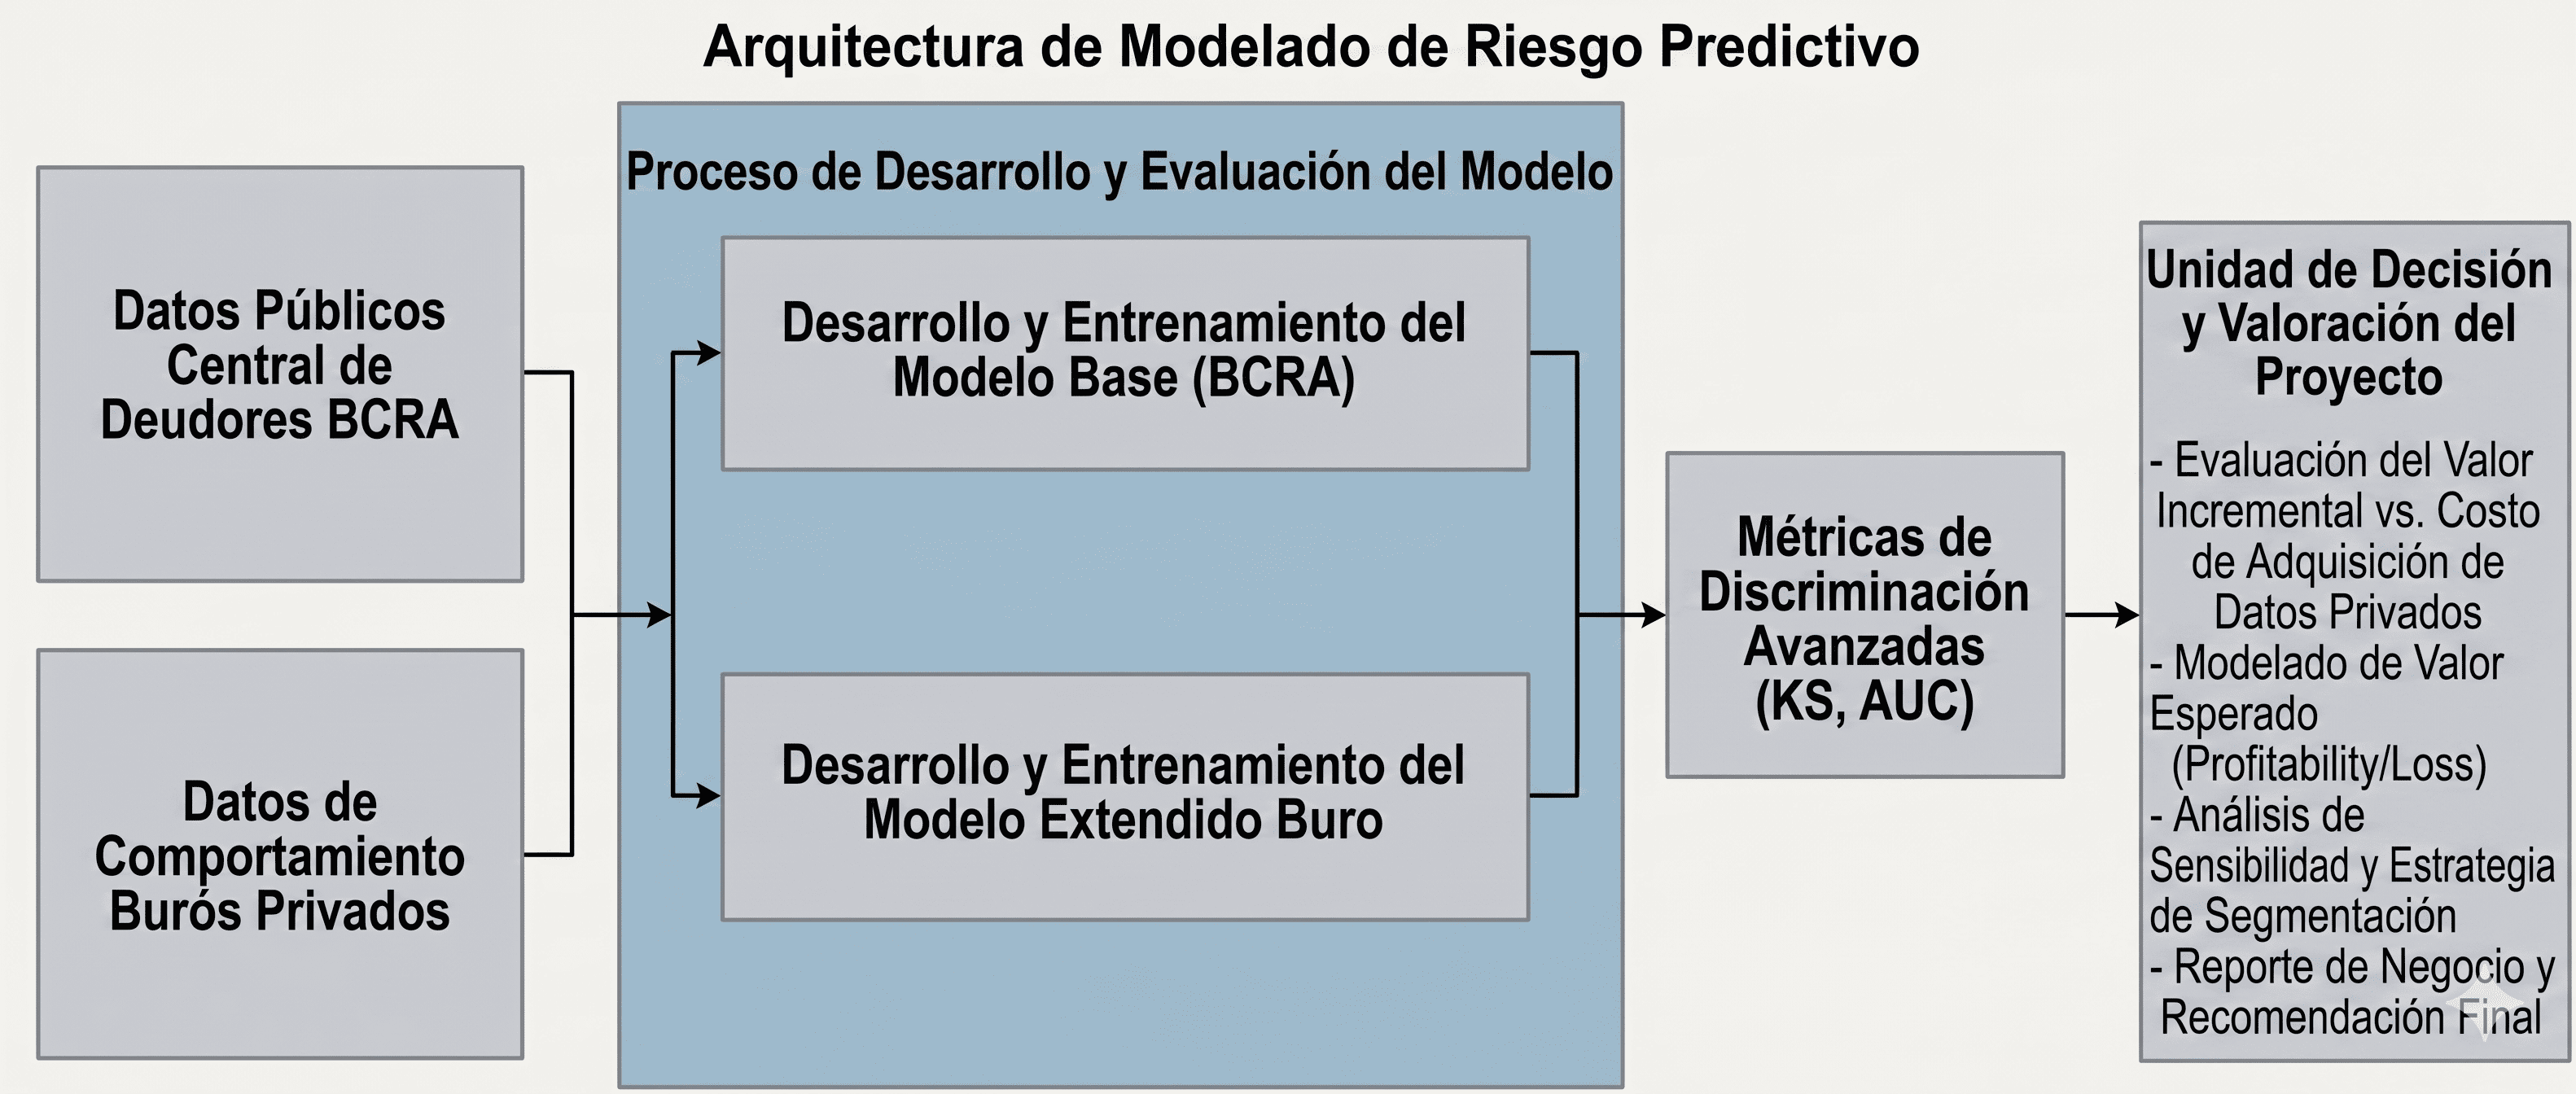
\includegraphics[width=.65\textwidth]{./Figuras/Modelado.png}
+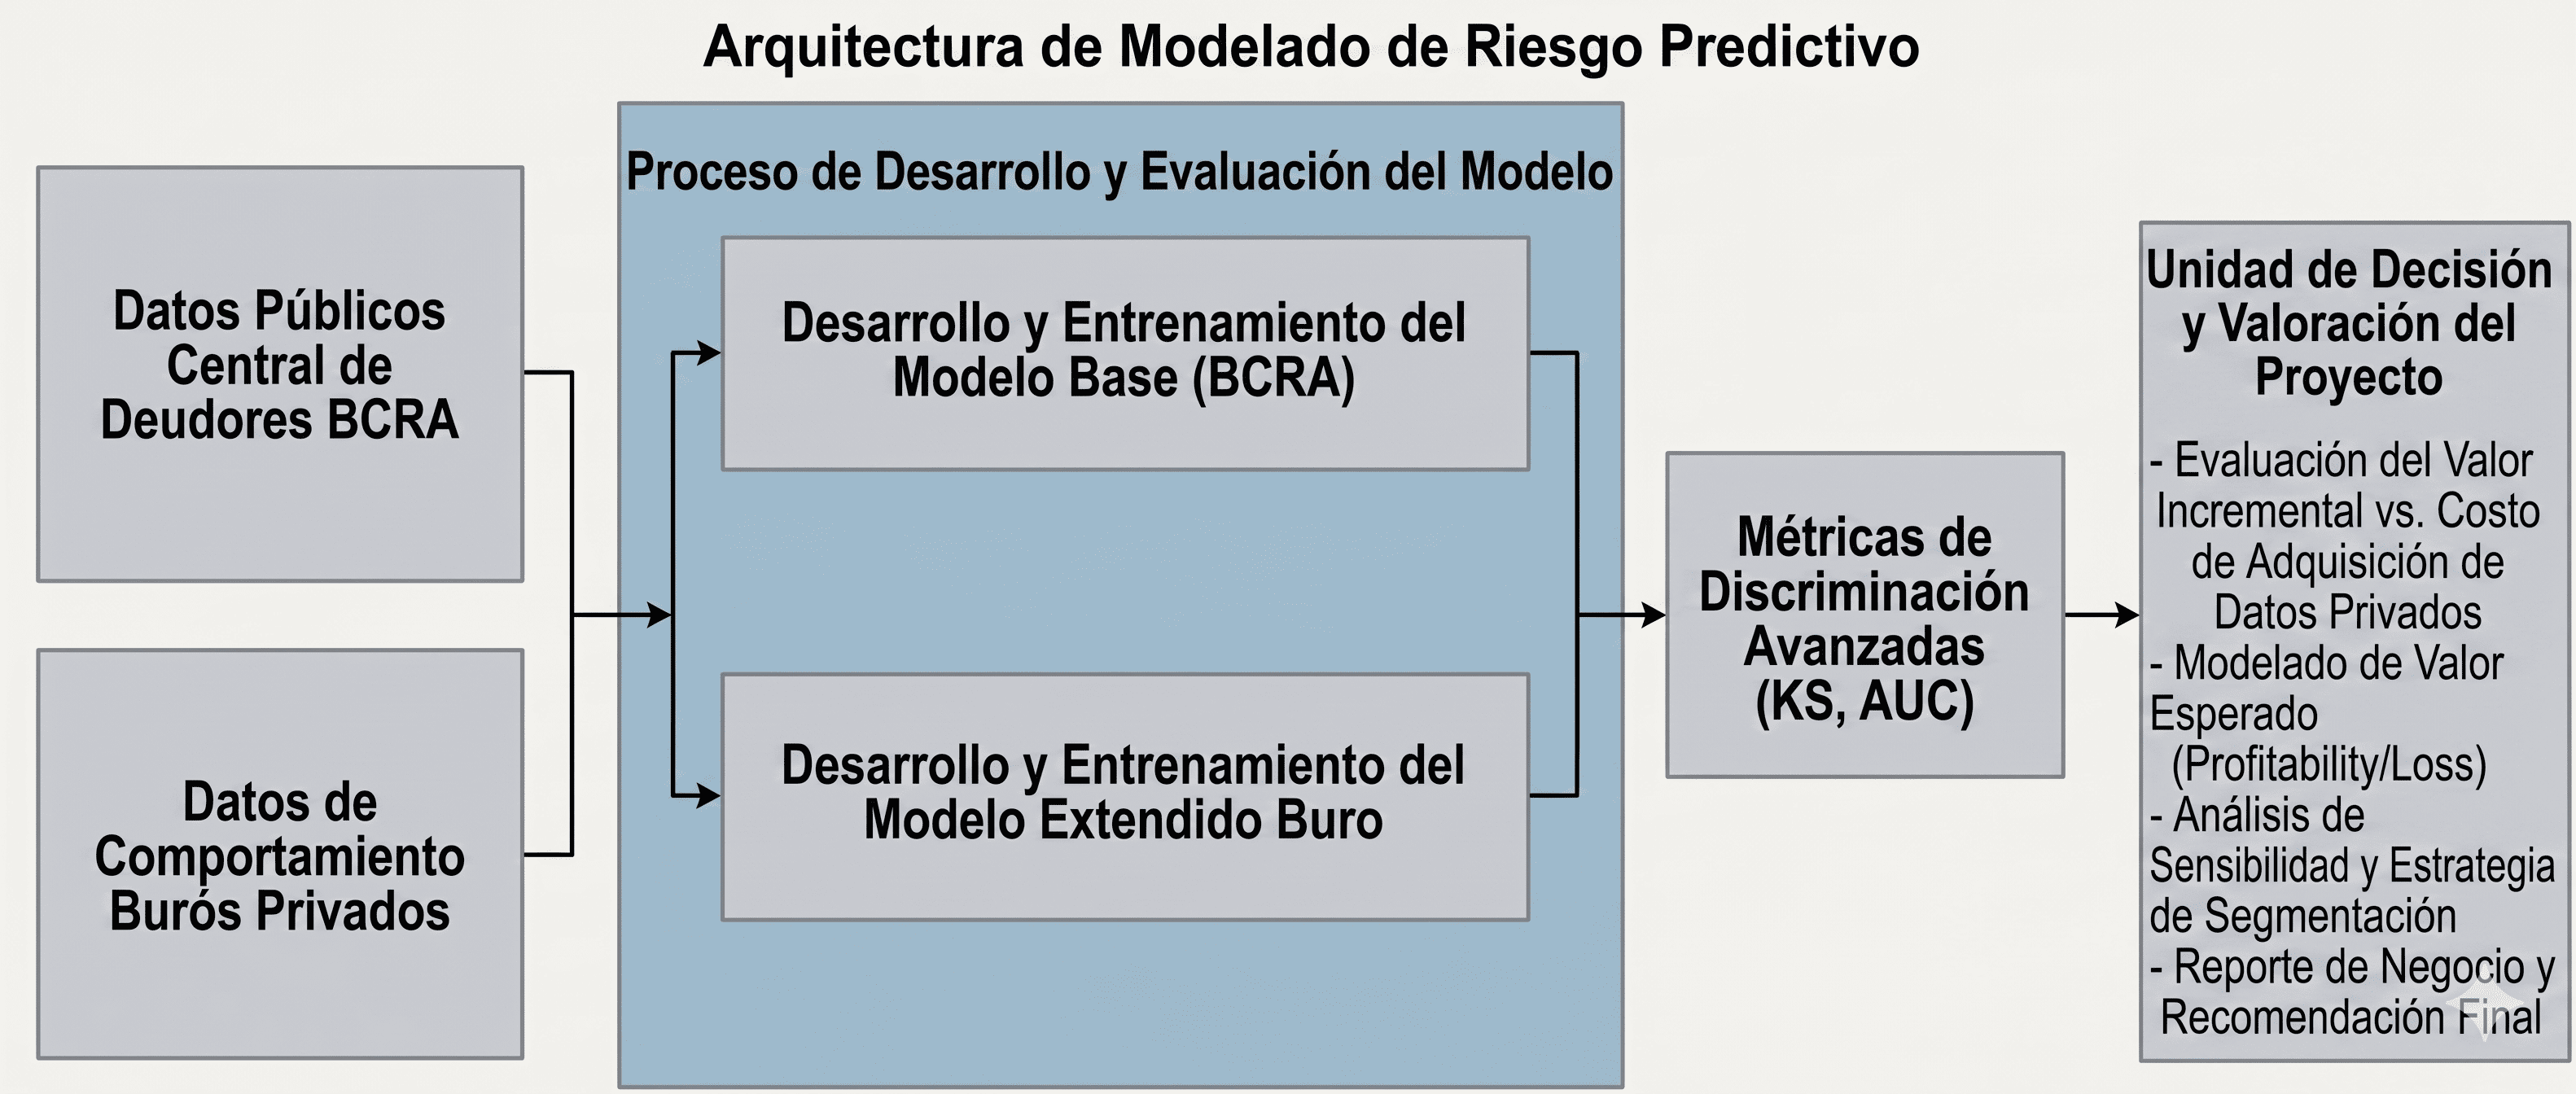
\includegraphics[width=.95\textwidth]{./Figuras/Modelado.png}
 \caption{Diagrama en bloques del sistema.}
 \label{fig:diagBloques}
 \end{figure}
@@ -123,12 +119,7 @@ La propuesta de valor de este proyecto consiste en desarrollar, entrenar y evalu
 \vspace{25px}
 
 
-\section{2. Identificación y análisis de los interesados}
-\label{sec:interesados}
-
-En el desarrollo de modelos predictivos de riesgo crediticio, la correcta identificación de los interesados resulta imperativa para garantizar que los requerimientos analíticos y las métricas de \textit{performance} se ajusten a la necesidad real del negocio. La propuesta de valor empírica de este proyecto exige una validación rigurosa por parte de los actores clave para contrastar el valor de la información de comportamiento del buró privado frente a los scores genéricos.
-
-\begin{table}[ht]
+\begin{table}[H]
 \caption{Identificación de los interesados}
 \label{tab:interesados}
 \begin{tabularx}{\linewidth}{@{}|l|X|X|l|@{}}
@@ -136,22 +127,15 @@ En el desarrollo de modelos predictivos de riesgo crediticio, la correcta identi
 \rowcolor[HTML]{C0C0C0}
 Rol & Nombre y Apellido & Organización & Puesto \\ \hline
 Cliente & John Doe & Nueva Compañía Financiera & Responsable de Riesgo \\ \hline
-Responsable & \authorname & FIUBA & Alumno \\ \hline
+Cliente Opositor & José Finanzas & Nueva Compañía Financiera & Responsable de Finanzas \\ \hline
+Seguridad & Pepe Governance & Nueva Compañía Financiera & Responsable de Gobernanza de Datos \\ \hline
+Responsable & \authorname & FIUBA & Científico de Datos \\ \hline
 Orientador & \supname & \pertesupname & Director del Trabajo Final \\ \hline
-Opositores & - & Nueva Compañía Financiera & Sector de Finanzas / Presupuesto \\ \hline
+Codirector & \cosupname & \pertecosupname & Codirector del Trabajo Final \\ \hline
+
 \end{tabularx}
 \end{table}
 
-A continuación, se detallan las principales características y expectativas metodológicas de cada interesado clave con relación al proyecto:
-
-\begin{itemize}
-\item \textbf{Cliente (John Doe):} Es el responsable directo que aprobará los resultados y validará el entregable final. Su evaluación se centrará empíricamente en corroborar si el enriquecimiento algorítmico con datos privados aporta un incremento estadísticamente significativo en la métrica del estadístico Kolmogorov-Smirnov (KS), justificando su viabilidad comercial frente a modelos puramente transaccionales.
-\item \textbf{Responsable (\authorname):} Ejerce la autoridad operativa y analítica para gestionar el ciclo de vida del proyecto, abarcando desde la recolección e imputación de variables, hasta la calibración de los hiperparámetros de los algoritmos de ensamble y la contrastación rigurosa de las distribuciones poblacionales.
-\item \textbf{Orientador (\supname):} Como experto técnico, supervisará el rigor académico de la experimentación y el diseño algorítmico. Se encargará de asegurar la correcta partición de conjuntos de validación, previniendo sesgos o el sobreajuste (\textit{overfitting}) en la comparación de las fuentes públicas y privadas.
-\item \textbf{Opositores (Sector de Finanzas / Presupuesto):} Representan al grupo interno de la entidad cliente que prioriza la reducción de costos operativos a corto plazo. Su oposición radica en considerar el proyecto financieramente oneroso, prefiriendo la utilización exclusiva de datos públicos del BCRA (CENDEU) por ser económicamente más viables, aun asumiendo un detrimento en la \textit{performance} predictiva. El rigor de esta investigación deberá refutar empíricamente su postura, demostrando que la mejora en la capacidad de discriminación (medida a través del KS) compensa holgadamente el costo de adquisición de los datos de buró.
-\end{itemize}
-
-
 \section{3. Propósito del proyecto}
 \label{sec:proposito}
 
@@ -195,294 +179,281 @@ Para el desarrollo del presente proyecto de investigación empírica se supone q
 \section{6. Requerimientos}
 \label{sec:requerimientos}
 
-\begin{consigna}{red} % ELIMINAR \begin{consigna}{red} y \end{consigna}{red} en las secciones que vayan completando para cada entrega parcial.
-Los requerimientos deben enumerarse y de ser posible estar agrupados por afinidad, por ejemplo:
-
 \begin{enumerate}
-	\item Requerimientos funcionales:
-		\begin{enumerate}
-			\item El sistema debe...
-			\item Tal componente debe...
-			\item El usuario debe poder...
-		\end{enumerate}
-	\item Requerimientos de documentación:
-		\begin{enumerate}
-			\item Requerimiento 1.
-			\item Requerimiento 2 (prioridad menor)
-		\end{enumerate}
-	\item Requerimiento de testing...
-	\item Requerimientos de la interfaz...
-	\item Requerimientos interoperabilidad...
-	\item etc...
+
+    \item \textbf{Requerimientos funcionales}
+    \begin{enumerate}
+        \item El sistema debe entrenar y evaluar modelos predictivos de riesgo crediticio experimentando con distintos algoritmos, aislando el rendimiento del modelo base (datos públicos del BCRA) respecto al modelo enriquecido (datos privados del buró).
+        \item El sistema debe predecir una variable objetivo (\textit{target} o marca de incumplimiento) definida taxativamente como la ocurrencia de un atraso de pago superior a 90 días en el transcurso de los 12 meses posteriores al punto de observación.
+        \item El sistema debe calcular y reportar obligatoriamente el estadístico Kolmogorov-Smirnov (KS) como métrica central para evaluar la capacidad del modelo para separar y discriminar las funciones de distribución de dos poblaciones mutuamente excluyentes: los buenos pagadores y los malos pagadores.
+        \item El cálculo de variables, la ingeniería de características (\textit{feature engineering}) y la predicción del modelo deben estructurarse para ser ejecutados en modalidad \textit{batch} sobre un conjunto dado de usuarios.
+    \end{enumerate}
+
+    \item \textbf{Requerimientos de datos a utilizar}
+    \begin{enumerate}
+        \item Los datos transaccionales extraídos del buró privado y del BCRA deben abarcar un período histórico definido estrictamente como los 60 meses hacia atrás desde el punto de observación, y procesarse en entornos que garanticen su anonimato y confidencialidad.
+        \item Cada usuario debe pertenecer de manera mutuamente excluyente a los conjuntos de entrenamiento, validación o prueba para evitar sesgos analíticos y filtración de información (\textit{data leakage}).
+        \item El conjunto de datos crediticios utilizado para entrenar los algoritmos no debe ser compartido públicamente bajo ninguna circunstancia, respetando el marco normativo vigente.
+    \end{enumerate}
+
+    \item \textbf{Requerimientos de documentación}
+    \begin{enumerate}
+        \item Se debe redactar una memoria técnica detallando la optimización de hiperparámetros y el análisis exploratorio realizado sobre los conjuntos de datos.
+        \item Se debe elaborar un informe que demuestre empíricamente el incremento porcentual del estadístico KS, justificando de manera cuantitativa la capacidad predictiva de los datos privados del buró frente al modelo base del BCRA.
+        \item Se debe analizar y documentar la importancia predictiva de las variables independientes (\textit{feature importance}) para garantizar la explicabilidad y transparencia del \textit{scoring} crediticio.
+    \end{enumerate}
+
 \end{enumerate}
 
-Leyendo los requerimientos se debe poder interpretar cómo será el proyecto y su funcionalidad.
+\section{7. Historias de usuarios (\textit{Product backlog})}
+\label{sec:backlog}
 
-Indicar claramente cuál es la prioridad entre los distintos requerimientos y si hay requerimientos opcionales. 
+Para la ponderación de las historias de usuario se utilizarán tres criterios, cada uno con tres niveles posibles de calificación:
 
-\textbf{¡¡¡No olvidarse de que los requerimientos incluyen a las regulaciones y normas vigentes!!!}
+\textbf{Dificultad}
+\begin{itemize}
+    \item Baja: 1 punto
+    \item Media: 3 puntos
+    \item Alta: 5 puntos
+\end{itemize}
 
-Y al escribirlos seguir las siguientes reglas:
+\textbf{Complejidad}
 \begin{itemize}
-	\item Ser breve y conciso (nadie lee cosas largas). 
-	\item Ser específico: no dejar lugar a confusiones.
-	\item Expresar los requerimientos en términos que sean cuantificables y medibles.
+    \item Baja: 2 puntos
+    \item Media: 5 puntos
+    \item Alta: 7 puntos
 \end{itemize}
 
-\end{consigna} % ELIMINAR \begin{consigna}{red} y \end{consigna}{red} en las secciones que vayan completando para cada entrega parcial.
+\textbf{Incertidumbre}
+\begin{itemize}
+    \item Baja: 1 punto
+    \item Media: 5 puntos
+    \item Alta: 10 puntos
+\end{itemize}
 
-\section{7. Historias de usuarios (\textit{Product backlog})}
-\label{sec:backlog}
+El puntaje final de cada historia de usuario será calculado como el número de la secuencia de Fibonacci más próximo mayor o igual a la suma de las calificaciones en los 3 criterios. A continuación, se detallan las historias agrupadas analíticamente por rol:
 
-\begin{consigna}{red}
-Descripción: en esta sección se deben incluir las historias de usuarios y su ponderación (\textit{history points}). Recordar que las historias de usuarios son descripciones cortas y simples de una característica contada desde la perspectiva de la persona que desea la nueva capacidad, generalmente un usuario o cliente del sistema. La ponderación es un número entero que representa el tamaño de la historia comparada con otras historias de similar tipo.
+\textbf{Rol: Científico de Datos}
+\begin{enumerate}
+    \item Como Científico de Datos quiero entrenar un modelo base con información pública del BCRA y un modelo enriquecido con información del buró privado para aislar y cuantificar el incremento del estadístico KS en la separación de buenos y malos pagadores. (5+7+5 = 17 $\rightarrow$ 21 puntos)
+    
+    \item Como Científico de Datos quiero ejecutar una validación cruzada en diferentes ventanas temporales (\textit{Out-of-Time validation}) para asegurar que la estabilidad de las métricas de separación poblacional se mantenga constante y no sufra volatilidad a causa del sobreajuste algorítmico. (3+7+5 = 15 $\rightarrow$ 21 puntos)
+\end{enumerate}
 
-Se debe indicar explícitamente el criterio para calcular los \textit{story points} de cada historia.
+\textbf{Rol: Analista de Riesgos}
+\begin{enumerate}\setcounter{enumi}{2}
+    \item Como Analista de Riesgos quiero comparar empíricamente la capacidad de discriminación de ambos modelos a través de todos los deciles de riesgo, validando la consistencia predictiva en toda la distribución poblacional para justificar cuantitativamente la adquisición de datos de comportamiento no regulado. (3+5+5 = 13 $\rightarrow$ 13 puntos)
+    
+    \item Como Analista de Riesgos quiero evaluar la importancia de las variables independientes (\textit{feature importance}) del modelo híbrido para comprender qué características del buró privado determinan el comportamiento crediticio y garantizar la interpretabilidad de la decisión algorítmica. (3+5+1 = 9 $\rightarrow$ 13 puntos)
+    
+    \item Como Analista de Riesgos quiero calcular el Índice de Estabilidad Poblacional (PSI) de las variables estructuradas del buró privado para garantizar que las distribuciones no sufran deriva de datos (\textit{Data Drift}) temporal frente a la muestra base, asegurando la robustez y vigencia del modelo. (3+5+1 = 9 $\rightarrow$ 13 puntos)
+\end{enumerate}
 
-El formato propuesto es: 
-\begin{enumerate}
-\item ``Como [rol] quiero [tal cosa] para [tal otra cosa]."
+\textbf{Rol: Analista de Finanzas}
+\begin{enumerate}\setcounter{enumi}{5}
+    \item Como Analista del Sector de Finanzas quiero evaluar las predicciones del modelo híbrido para aumentar la cantidad de usuarios aprobados manteniendo el mismo porcentaje de malos pagadores de la cartera actual (\textit{estrategia de swap-in}), demostrando así la viabilidad comercial y operativa de la información externa. (3+5+1 = 9 $\rightarrow$ 13 puntos)
+\end{enumerate}
 
-\textit{Story points}: 8 (complejidad: 3, dificultad: 2, incertidumbre: 3)
+\textbf{Rol: Gobernanza de Datos}
+\begin{enumerate}\setcounter{enumi}{6}
+    \item Como Responsable del área de Gobernanza de Datos quiero validar los \textit{pipelines} de preprocesamiento de características transaccionales para asegurar la anonimización de la información privada, certificando el cumplimiento de la Ley 25.326 de Protección de Datos Personales. (1+2+5 = 8 $\rightarrow$ 8 puntos)
 \end{enumerate}
-\end{consigna}
 
 \section{8. Entregables principales del proyecto}
 \label{sec:entregables}
 
-\begin{consigna}{red}
-Los entregables del proyecto son (ejemplo):
-
+Los entregables principales del proyecto son:
 \begin{itemize}
-	\item Manual de usuario.
-	\item Diagrama de circuitos esquemáticos.
-	\item Código fuente del firmware.
-	\item Diagrama de instalación.
-	\item Memoria del trabajo final.
-	\item etc...
+    \item Memoria técnica del Trabajo Final, documentando la fundamentación empírica, la ingeniería de características y la justificación matemática del incremento en el estadístico Kolmogorov-Smirnov (KS) entre el modelo base (BCRA) y el modelo híbrido, omitiendo cualquier exposición de datos sensibles.
+    \item Informe ejecutivo orientado al Sector de Finanzas, detallando de forma clara y directa el beneficio comercial del proyecto. Este documento demostrará empíricamente cómo el uso de los datos del buró permite aumentar la cantidad de usuarios aprobados manteniendo constante el porcentaje de malos pagadores en la cartera.
+    \item \textit{Jupyter Notebooks} y \textit{pipeline} de procesamiento de datos. El código fuente no será entregado bajo ningún formato; por políticas de confidencialidad, únicamente estará disponible de forma exclusiva en un repositorio institucional privado.
 \end{itemize}
-\end{consigna}
 
 \section{9. Desglose del trabajo en tareas}
 \label{sec:wbs}
 
-\begin{consigna}{red}
-El WBS debe tener relación directa o indirecta con los requerimientos.  Son todas las actividades que se harán en el proyecto para dar cumplimiento a los requerimientos. Se recomienda mostrar el WBS mediante una lista indexada:
+A continuación se detalla la Estructura de Desglose del Trabajo (EDT/WBS), donde cada paquete de trabajo ha sido descompuesto en tareas técnicas de duración no mayor a 40 horas para garantizar un seguimiento riguroso. El esfuerzo total estimado para este proyecto de modelado predictivo es de 620 horas.
 
 \begin{enumerate}
-\item Grupo de tareas 1 (suma h)
-	\begin{enumerate}
-	\item Tarea 1 (tantas h)
-	\item Tarea 2 (tantas h)
-	\item Tarea 3 (tantas h)
-	\end{enumerate}
-\item Grupo de tareas 2 (suma h)
-	\begin{enumerate}
-	\item Tarea 1 (tantas h)
-	\item Tarea 2 (tantas h)
-	\item Tarea 3 (tantas h)
-	\end{enumerate}
-\item Grupo de tareas 3 (suma h)
-	\begin{enumerate}
-	\item Tarea 1 (tantas h)
-	\item Tarea 2 (tantas h)
-	\item Tarea 3 (tantas h)
-	\item Tarea 4 (tantas h)
-	\item Tarea 5 (tantas h)
-	\end{enumerate}
+
+    \item \textbf{Estudio de la temática y marco normativo (100 h)}
+    \begin{enumerate}
+        \item Lectura de bibliografía sobre modelos de ensamble aplicados a \textit{scoring} crediticio (40 h).
+        \item Relevamiento del marco normativo (Ley 25.326) y pautas de gobernanza de datos para el anonimato (20 h).
+        \item Exploración documental de la estructura de diccionarios de variables del BCRA (CENDEU) y del buró privado (40 h).
+    \end{enumerate}
+
+    \item \textbf{Definición de lineamientos del modelo (70 h)}
+    \begin{enumerate}
+        \item Formulación metodológica para la evaluación de la separación poblacional y umbrales del estadístico KS (40 h).
+        \item Validación y ajuste de la propuesta analítica y métricas de éxito con el Sector de Finanzas (30 h).
+    \end{enumerate}
+
+    \item \textbf{Obtención y preprocesamiento de datos (140 h)}
+    \begin{enumerate}
+        \item Desarrollo de la consulta estructurada para la extracción de la ventana de observación histórica de 60 meses (40 h).
+        \item Integración de los datos tabulares públicos (BCRA) con los datos externos (buró privado) garantizando anonimato (40 h).
+        \item Definición y etiquetado de la variable objetivo (\textit{target}): atraso mayor a 90 días en la ventana de desempeño de 12 meses (30 h).
+        \item Limpieza exhaustiva de la muestra, tratamiento de valores nulos y filtrado de \textit{outliers} (30 h).
+    \end{enumerate}
+
+    \item \textbf{Desarrollo algorítmico y evaluación (210 h)}
+    \begin{enumerate}
+        \item Análisis exploratorio de datos (EDA) y cálculo de la divergencia de distribuciones (30 h).
+        \item Ingeniería de características (\textit{feature engineering}) y selección iterativa de variables predictivas (40 h).
+        \item Partición de la muestra y entrenamiento secuencial del modelo base y el modelo enriquecido (40 h).
+        \item Cálculo del Índice de Estabilidad Poblacional (PSI) y evaluación del peso predictivo de variables (\textit{feature importance}) (30 h).
+        \item Cálculo y análisis comparativo del incremento del estadístico Kolmogorov-Smirnov (KS) en todos los deciles de riesgo (40 h).
+        \item Armado del \textit{pipeline} definitivo para la productivización \textit{batch} y estimación de viabilidad comercial (\textit{swap-in}) (30 h).
+    \end{enumerate}
+
+    \item \textbf{Documentación y cierre del proyecto (100 h)}
+    \begin{enumerate}
+        \item Redacción de la memoria técnica documentando la experimentación empírica (60 h).
+        \item Elaboración del informe ejecutivo analítico orientado al área de presupuesto y finanzas (20 h).
+        \item Preparación del material audiovisual y simulacro para la defensa pública del trabajo (20 h).
+    \end{enumerate}
+
 \end{enumerate}
 
-Cantidad total de horas: tantas.
 
-\textbf{¡Importante!:} la unidad de horas es h y va separada por espacio del número. Es incorrecto escribir ``23hs".
+\begin{consigna}{red}
+\section{10. Planificación de Sprints}
 
-\textbf{Se recomienda que no haya ninguna tarea que lleve más de 40 h.} De ser así se recomienda dividirla en tareas de menor duración.
+Organizar las tareas técnicas del proyecto en sprints de trabajo que permitan distribuir de forma equilibrada la carga horaria total, estimada en 600 horas.
 
-\end{consigna}
+\textbf{Consigna:}
+\begin{itemize}
+  \item Completar una tabla que relacione sprints con HU y tareas técnicas correspondientes.
+  \item Incluir estimación en horas para cada tarea.
+  \item Indicar responsable y porcentaje de avance estimado o completado.
+  \item Contemplar también tareas de planificación, documentación, redacción de memoria y preparación de defensa.
+\end{itemize}
 
-\section{10. Diagrama de Activity On Node}
-\label{sec:AoN}
+\textbf{Conceptos clave:}
+\begin{itemize}
+  \item Una \'{e}pica es una unidad funcional amplia; una historia de usuario es una funcionalidad concreta; un sprint es una unidad de tiempo donde se ejecutan tareas.
+  \item Las tareas son el nivel más desagregado: permiten estimar tiempos, asignar responsables y monitorear progreso.
+\end{itemize}
 
-\begin{consigna}{red}
-Armar el AoN a partir del WBS definido en la etapa anterior.
+\textbf{Duración sugerida:}
+\begin{itemize}
+  \item Para un proyecto de 600 h, se recomienda planificar entre 10 y 12 sprints de aproximadamente 2 semanas cada uno.
+  \item Asignar entre 45 y 50 horas efectivas por sprint a tareas técnicas.
+  \item Reservar 100 a 120 h para actividades no técnicas (planificación, escritura, reuniones, defensa).
+\end{itemize}
 
-Una herramienta simple para desarrollar los diagramas es el Draw.io (\url{https://app.diagrams.net/}).
-\href{https://app.diagrams.net}{Draw.io}
+\textbf{Importante:}
+\begin{itemize}
+  \item En proyectos individuales, el responsable suele ser el propio autor.
+  \item Aun así, desagregar tareas facilita el seguimiento y mejora continua.
+\end{itemize}
 
+\textbf{Conversión opcional de Story Points a horas:}
+\begin{itemize}
+  \item 1 SP \(\approx\) 2 h como referencia flexible.
+  \item Tener en cuenta aproximaciones tipo Fibonacci.
+\end{itemize}
 
-\begin{figure}[htpb]
-\centering 
-\includegraphics[width=.8\textwidth]{./Figuras/AoN.png}
-\caption{Diagrama de \textit{Activity on Node}.}
-\label{fig:AoN}
-\end{figure}
+\begin{table}[htpb]
+\centering
+\caption{Formato sugerido}
+\begin{tabularx}{\linewidth}{@{}|l|l|X|c|l|c|@{}}
+\hline
+\rowcolor[HTML]{C0C0C0}
+Sprint & HU o fase & Tarea & Horas / SP & Responsable & \% Completado \\ \hline
+Sprint 0 & Planificación & Definir alcance y cronograma & 10 h & Alumno & 100\% \\ \hline
+Sprint 0 & Planificación & Reunión con el tutor/cliente & 5 h & Alumno & 50\% \\ \hline
+Sprint 0 & Planificación & Ajuste de los entregables & 6 h & Alumno & 25\% \\ \hline
+Sprint 1 & HU1 & Tarea 1 HU1 & 6 h / 3 SP & Alumno & 0\% \\ \hline
+Sprint 1 & HU1 & Tarea 2 HU1 & 10 h / 5 SP & Alumno & 0\% \\ \hline
+Sprint 2 & HU2 & Tarea 1 HU2 & 7 h / 5 SP & Alumno & 0\% \\ \hline
+... & ... & ... & ... & ... & ... \\ \hline
+Sprint 5 & Escritura & Redacción memoria & 50 h / 34 SP & Alumno & 0\% \\ \hline
+Sprint 6 & Defensa & Preparación de la exposición & 20 h / 13 SP & Alumno & 0\% \\ \hline
+\end{tabularx}
+\end{table}
 
-Indicar claramente en qué unidades están expresados los tiempos.
-De ser necesario indicar los caminos semi críticos y analizar sus tiempos mediante un cuadro.
-Es recomendable usar colores y un cuadro indicativo describiendo qué representa cada color.
+\textbf{Recomendaciones:}
+\begin{itemize}
+  \item Verificar que la carga horaria por sprint sea equilibrada.
+  \item Usar sprints de 1 a 3 semanas, acordes al cronograma general.
+  \item Actualizar el \% completado durante el seguimiento del proyecto.
+  \item Considerar un sprint final exclusivo para pruebas, revisión y ajustes antes de la defensa.
+\end{itemize}
 
-\end{consigna}
 
-\section{11. Diagrama de Gantt}
+\section{11. Diagrama de Gantt (sprints)}
 \label{sec:gantt}
 
-\begin{consigna}{red}
-Existen muchos programas y recursos \textit{online} para hacer diagramas de Gantt, entre los cuales destacamos:
+Visualizar en un diagrama de Gantt la planificación temporal del proyecto, tomando como base los sprints definidos en la sección anterior. Debe contemplar todas las horas del proyecto.
+
+Consigna:
 
 \begin{itemize}
-\item Planner
-\item GanttProject
-\item Trello + \textit{plugins}. En el siguiente link hay un tutorial oficial: \\ \url{https://blog.trello.com/es/diagrama-de-gantt-de-un-proyecto}
-\item Creately, herramienta online colaborativa. \\\url{https://creately.com/diagram/example/ieb3p3ml/LaTeX}
-\item Se puede hacer en latex con el paquete \textit{pgfgantt}\\ \url{http://ctan.dcc.uchile.cl/graphics/pgf/contrib/pgfgantt/pgfgantt.pdf}
+
+\item Elaborar un diagrama de Gantt que muestre la secuencia temporal de los sprints.
+
+\item Cada fila debe representar un sprint (con su número o nombre), y el eje horizontal debe indicar el tiempo (en semanas o fechas concretas).
+
+\item Las tareas técnicas derivadas de HU deben diferenciarse visualmente (por ejemplo, con un color distinto) de las tareas no técnicas (planificación, redacción, defensa).
+
+\item Incluir todas las tareas estimadas en cada sprint.
 \end{itemize}
 
-Pegar acá una captura de pantalla del diagrama de Gantt, cuidando que la letra sea suficientemente grande como para ser legible. 
-Si el diagrama queda demasiado ancho, se puede pegar primero la ``tabla'' del Gantt y luego pegar la parte del diagrama de barras del diagrama de Gantt.
+Recomendaciones para el Gantt:
 
-Configurar el software para que en la parte de la tabla muestre los códigos del EDT (WBS).\\
-Configurar el software para que al lado de cada barra muestre el nombre de cada tarea.\\
-Revisar que la fecha de finalización coincida con lo indicado en el Acta Constitutiva.
+\begin{itemize}
 
-En la figura \ref{fig:gantt}, se muestra un ejemplo de diagrama de gantt realizado con el paquete de \textit{pgfgantt}. 
-En la plantilla pueden ver el código que lo genera y usarlo de base para construir el propio.
+	\item Podés usar herramientas gratuitas como TeamGantt, ClickUp, GanttProject, [Google Sheets], [Trello + Planyway], entre otras.
+	\item Ordená los sprints de forma cronológica, comenzando con Sprint 0 (planificación) y finalizando con el sprint de defensa.
+	\item Asegurate de reflejar la duración realista de cada sprint según tu disponibilidad y el cronograma general del posgrado.
+	\item Incluí hitos importantes: reuniones, entregas parciales, defensa.
+\end{itemize}
 
-Las fechas pueden ser calculadas utilizando alguna de las herramientas antes citadas. Sin embargo, el siguiente ejemplo
-fue elaborado utilizando 
-\href{https://docs.google.com/spreadsheets/d/1fBz8NhSpc4tkkhz3KjJCbh1nR_ltDkfEcZi4tZXduqs}{esta hoja de cálculo}.
 
-Es importante destacar que el ancho del diagrama estará dado por la longitud del texto utilizado para las tareas 
-(Ejemplo: tarea 1, tarea 2, etcétera) y el valor \textit{x unit}. Para mejorar la apariencia del diagrama, es necesario
-ajustar este valor y, quizás, acortar los nombres de las tareas.
+Incluir una imagen legible del diagrama de Gantt. Si es muy ancho, presentar primero la tabla y luego el gráfico de barras.
 
-\begin{figure}[htpb]
-  \begin{center}
-    \begin{ganttchart}[
-      time slot unit=day,
-      time slot format=isodate,
-      x unit=0.038cm,
-      y unit title=0.7cm,
-      y unit chart=0.6cm,
-      milestone/.append style={xscale=4}
-      ]{2021-03-05}{2021-12-16}
-      \gantttitlecalendar*{2021-03-05}{2021-12-16}{year} \\
-      \gantttitlecalendar*{2021-03-05}{2021-12-16}{month} \\
-      \ganttgroup{Duración Total}{2021-03-05}{2021-12-16} \\
-      %%%%%%%%%%%%%%%%%Organización
-      \ganttgroup{Organización}{2021-03-05}{2021-04-16} \\
-      \ganttbar{Planificación del proyecto}{2021-03-05}{2021-04-15} \\
-      %%%%%%%%%%%%%%%%%Ejecución
-      \ganttgroup{Ejecución}{2021-04-16}{2021-10-21} \\
-      \ganttbar{Tarea 1}{2021-04-16}{2021-04-29} \\
-      \ganttbar{Tarea 2}{2021-04-30}{2021-05-13} \\
-      \ganttbar{Tarea 3}{2021-05-14}{2021-05-27} \\
-      \ganttbar{Tarea 4}{2021-05-28}{2021-07-12} \\
-      \ganttbar{Tarea 5}{2021-07-13}{2021-08-09} \\
-      \ganttbar{Tarea 6}{2021-08-10}{2021-09-23} \\
-      \ganttbar{Tarea 7}{2021-09-24}{2021-09-30} \\
-      \ganttbar{Tarea 8}{2021-10-01}{2021-10-14} \\
-      \ganttbar{Tarea 9}{2021-10-15}{2021-10-21} \\
-      % %%%%%%%%%%%%%%%%%Finalización
-      \ganttgroup{Finalización}{2021-10-22}{2021-12-16} \\
-      \ganttbar{Memoria v1}{2021-10-22}{2021-11-04} \\
-      \ganttbar{Memoria v2}{2021-11-05}{2021-11-18} \\
-      \ganttbar{Memoria final}{2021-11-19}{2021-12-02} \\
-      % La fecha del siguiente milestone es la fecha en que terminamos la memoria
-      \ganttmilestone{Enviar memoria al director}{2021-12-02} \\
-      \ganttbar{Elaborar la presentación}{2021-12-03}{2021-12-16} \\
-      \ganttmilestone{Ensayo de la presentación}{2021-12-16} \\
-      %%%%%%%%%%%%%%%%%%%%%%%%%%%%%%%%%%%%%%%%%%%%%%%%%%%%%%%%%%%%%%%
-    \end{ganttchart}
-  \end{center}
-  \caption{Diagrama de gantt de ejemplo}
-  \label{fig:gantt}
-\end{figure}
 
 
-\begin{landscape}
-\begin{figure}[htpb]
-\centering 
-\includegraphics[height=.85\textheight]{./Figuras/Gantt-2.png}
-\caption{Ejemplo de diagrama de Gantt (apaisado).} %Modificar este título acorde.
-\label{fig:diagGantt}
-\end{figure}
+\section{12. Gobernanza de datos}
+\label{sec:gobernanza}
 
-\end{landscape}
+En esta sección se debe analizar de manera integral el marco normativo y ético asociado al uso de los datos y al desarrollo de soluciones basadas en inteligencia artificial.
 
-\end{consigna}
+El análisis se divide en dos partes:
 
+\begin{itemize}
+  \item Cumplimiento normativo.
+  \item Ética en el uso de inteligencia artificial.
+\end{itemize}
 
-\section{12. Presupuesto detallado del proyecto}
-\label{sec:presupuesto}
+\subsection{Cumplimiento normativo}
+Este análisis es clave para garantizar el cumplimiento normativo y evitar conflictos legales durante el desarrollo y publicación del proyecto.
+
+En esta subsección se debe identificar si los datos utilizados en el proyecto están sujetos a normativas de protección de datos y privacidad, y en qué condiciones pueden emplearse.
+
+Aspectos a considerar:
 
-\begin{consigna}{red}
-Si el proyecto es complejo entonces separarlo en partes:
 \begin{itemize}
-	\item Un total global, indicando el subtotal acumulado por cada una de las áreas.
-	\item El desglose detallado del subtotal de cada una de las áreas.
+  \item Determinar si los datos están regulados por normativas como el GDPR, la Ley 25.326 de Protección de Datos Personales (Argentina), la HIPAA u otras, según la jurisdicción o la temática del proyecto.
+  \item Aclarar si las fuentes de datos son propias, de acceso público o licenciadas. En este último caso, explicitar la licencia correspondiente y sus condiciones de uso. Realizar este mismo análisis para las herramientas y, en caso de corresponder, para los modelos preentrenados a emplear.
+  \item Analizar la viabilidad legal del proyecto, considerando los mecanismos necesarios para garantizar el cumplimiento normativo y la trazabilidad de los datos.
 \end{itemize}
 
-IMPORTANTE: No olvidarse de considerar los COSTOS INDIRECTOS.
+\subsection{Ética en el uso de inteligencia artificial}
 
-Incluir la aclaración de si se emplea como moneda el peso argentino (ARS) o si se usa moneda extranjera (USD, EUR, etc). Si es en moneda extranjera se debe indicar la tasa de conversión respecto a la moneda local en una fecha dada.
+En esta subsección se debe reflexionar sobre los aspectos éticos vinculados al uso de datos y algoritmos de inteligencia artificial. Se espera una evaluación de la integridad del sistema y su impacto social.
 
-\end{consigna}
+Aspectos a considerar:
 
-\begin{table}[htpb]
-\centering
-\begin{tabularx}{\linewidth}{@{}|X|c|r|r|@{}}
-\hline
-\rowcolor[HTML]{C0C0C0} 
-\multicolumn{4}{|c|}{\cellcolor[HTML]{C0C0C0}COSTOS DIRECTOS} \\ \hline
-\rowcolor[HTML]{C0C0C0} 
-Descripción &
-  \multicolumn{1}{c|}{\cellcolor[HTML]{C0C0C0}Cantidad} &
-  \multicolumn{1}{c|}{\cellcolor[HTML]{C0C0C0}Valor unitario} &
-  \multicolumn{1}{c|}{\cellcolor[HTML]{C0C0C0}Valor total} \\ \hline
- &
-  \multicolumn{1}{c|}{} &
-  \multicolumn{1}{c|}{} &
-  \multicolumn{1}{c|}{} \\ \hline
- &
-  \multicolumn{1}{c|}{} &
-  \multicolumn{1}{c|}{} &
-  \multicolumn{1}{c|}{} \\ \hline
-\multicolumn{1}{|l|}{} &
-   &
-   &
-   \\ \hline
-\multicolumn{1}{|l|}{} &
-   &
-   &
-   \\ \hline
-\multicolumn{3}{|c|}{SUBTOTAL} &
-  \multicolumn{1}{c|}{} \\ \hline
-\rowcolor[HTML]{C0C0C0} 
-\multicolumn{4}{|c|}{\cellcolor[HTML]{C0C0C0}COSTOS INDIRECTOS} \\ \hline
-\rowcolor[HTML]{C0C0C0} 
-Descripción &
-  \multicolumn{1}{c|}{\cellcolor[HTML]{C0C0C0}Cantidad} &
-  \multicolumn{1}{c|}{\cellcolor[HTML]{C0C0C0}Valor unitario} &
-  \multicolumn{1}{c|}{\cellcolor[HTML]{C0C0C0}Valor total} \\ \hline
-\multicolumn{1}{|l|}{} &
-   &
-   &
-   \\ \hline
-\multicolumn{1}{|l|}{} &
-   &
-   &
-   \\ \hline
-\multicolumn{1}{|l|}{} &
-   &
-   &
-   \\ \hline
-\multicolumn{3}{|c|}{SUBTOTAL} &
-  \multicolumn{1}{c|}{} \\ \hline
-\rowcolor[HTML]{C0C0C0}
-\multicolumn{3}{|c|}{TOTAL} &
-   \\ \hline
-\end{tabularx}%
-\end{table}
+\begin{itemize}
+	\item Identificar posibles sesgos en los datos o modelos (ideológicos, culturales, de género, geográficos, etc.) y analizar sus consecuencias (por ejemplo: discriminación, manipulación, pérdida de privacidad o desinformación).
+	\item Analizar los posibles riesgos en términos de impacto social del uso indebido de la solución a desarrollar.
+	\item En caso de corresponder, proponer medidas de mitigación y mecanismos de confianza (auditorías, documentación, trazabilidad, revisión humana, etc.).
+	\item Finalmente, elaborar una reflexión general sobre la ética del proyecto, considerando tanto la equidad y transparencia del sistema como su impacto potencial en la sociedad.
+
+\end{itemize}
 
 
 \section{13. Gestión de riesgos}
@@ -555,46 +526,94 @@ Riesgo 3: plan de mitigación (si por el RPN fuera necesario elaborar un plan de
 
 \end{consigna}
 
+\section{14. Sprint Review}
+\label{sec:sprint_review}
 
-\section{14. Gestión de la calidad}
-\label{sec:calidad}
+La revisión de sprint (\emph{Sprint Review}) es una práctica fundamental en metodologías ágiles. Consiste en revisar y evaluar lo que se ha completado al finalizar un sprint. En esta instancia, se presentan los avances y se verifica si las funcionalidades cumplen con los criterios de aceptación establecidos. También se identifican entregables parciales y se consideran ajustes si es necesario.
 
-\begin{consigna}{red}
-Elija al menos diez requerimientos que a su criterio sean los más importantes/críticos/que aportan más valor y para cada uno de ellos indique las acciones de verificación y validación que permitan asegurar su cumplimiento.
+Aunque el proyecto aún se encuentre en etapa de planificación, esta sección permite proyectar cómo se evaluarán las funcionalidades más importantes del backlog. Esta mirada anticipada favorece la planificación enfocada en valor y permite reflexionar sobre posibles obstáculos.
 
-\begin{itemize} 
-\item Req \#1: copiar acá el requerimiento con su correspondiente número.
+\textbf{Objetivo:} anticipar cómo se evaluará el avance del proyecto a medida que se desarrollen las funcionalidades, utilizando como base al menos cuatro historias de usuario del \emph{Product Backlog}.
+
+
+Seleccionar al menos 4 HU del Product Backlog. Para cada una, completar la siguiente tabla de revisión proyectada:
+
+\textbf{Formato sugerido:}
+\begin{table}[htpb]
+\renewcommand{\arraystretch}{1.5}
+\begin{tabular}{|>{\raggedright\arraybackslash}m{2.4cm}|
+                >{\raggedright\arraybackslash}m{2.3cm}|
+                >{\raggedright\arraybackslash}m{3cm}|
+                >{\raggedright\arraybackslash}m{3cm}|
+                >{\raggedright\arraybackslash}m{3cm}|}
+\hline
+\rowcolor[HTML]{CCCCCC}
+\textbf{HU seleccionada} & \textbf{Tareas asociadas} & \textbf{Entregable esperado} & \textbf{¿Cómo sabrás que está cumplida?} & \textbf{Observaciones o riesgos} \\
+\hline
+                         & Tarea 1 &                             &                                           &                                     \\ \cline{2-2}
+\multirow{-2}{=}{HU1}    & Tarea 2 & \multirow{-2}{=}{Módulo funcional} & \multirow{-2}{=}{Cumple criterios de aceptación definidos} & \multirow{-2}{=}{Falta validar con el tutor} \\
+\hline
+                         & Tarea 1 &                             &                                           &                                     \\ \cline{2-2}
+\multirow{-2}{=}{HU3}    & Tarea 2 & \multirow{-2}{=}{Reporte generado} & \multirow{-2}{=}{Exportación disponible y clara} & \multirow{-2}{=}{Requiere datos reales} \\
+\hline
+                         & Tarea 1 &                             &                                           &                                     \\ \cline{2-2}
+\multirow{-2}{=}{HU5}    & Tarea 2 & \multirow{-2}{=}{Panel de gestión} & \multirow{-2}{=}{Roles diferenciados operativos} & \multirow{-2}{=}{Riesgo en integración} \\
+\hline
+                         & Tarea 1 &                             &                                           &                                     \\ \cline{2-2}
+\multirow{-2}{=}{HU7}    & Tarea 2 & \multirow{-2}{=}{Informe trimestral} & \multirow{-2}{=}{PDF con gráficos y evolución} & \multirow{-2}{=}{Puede faltar tiempo para ajustes} \\
+\hline
+\end{tabular}
+\end{table}
+
+\section{15. Sprint Retrospective}    
+\label{sec:sprint_retro}
+
+La retrospectiva de sprint es una práctica orientada a la mejora continua. Al finalizar un sprint, el equipo (o el alumno, si trabaja de forma individual) reflexiona sobre lo que funcionó bien, lo que puede mejorarse y qué acciones concretas pueden implementarse para trabajar mejor en el futuro.
+
+Durante la cursada se propuso el uso de la \textbf{Estrella de la Retrospectiva}, que organiza la reflexión en torno a cinco ejes:
 
 \begin{itemize}
-	\item Verificación para confirmar si se cumplió con lo requerido antes de mostrar el sistema al cliente. Detallar.
-	\item Validación con el cliente para confirmar que está de acuerdo en que se cumplió con lo requerido. Detallar. 
+\item  ¿Qué hacer más?
+\item  ¿Qué hacer menos?
+\item  ¿Qué mantener?
+\item  ¿Qué empezar a hacer?
+\item  ¿Qué dejar de hacer?
 \end{itemize}
 
-\end{itemize}
+Aun en una etapa temprana, esta herramienta permite que el alumno planifique su forma de trabajar, identifique anticipadamente posibles dificultades y diseñe estrategias de organización personal.
 
-Tener en cuenta que en este contexto se pueden mencionar simulaciones, cálculos, revisión de hojas de datos, consulta con expertos, mediciones, etc.  
+\textbf{Objetivo:} reflexionar sobre las condiciones iniciales del proyecto, identificando fortalezas, posibles dificultades y estrategias de mejora, incluso antes del inicio del desarrollo.
 
-Las acciones de verificación suelen considerar al entregable como ``caja blanca'', es decir se conoce en profundidad su funcionamiento interno.  
 
-En cambio, las acciones de validación suelen considerar al entregable como ``caja negra'', es decir, que no se conocen los detalles de su funcionamiento interno.
+Completar la siguiente tabla tomando como referencia los cinco ejes de la Estrella de la Retrospectiva (\emph{Starfish} o estrella de mar). Esta instancia te ayudará a definir buenas prácticas desde el inicio y prepararte para enfrentar el trabajo de forma organizada y flexible. Se deberá completar la tabla al menos para 3 sprints técnicos y 1 no técnico.
 
-\end{consigna}
+\textbf{Formato sugerido:}
 
-\section{15. Procesos de cierre}    
-\label{sec:cierre}
+\begin{table}[htpb]
+\renewcommand{\arraystretch}{1.4}
+\begin{tabular}{|>{\raggedright\arraybackslash}p{1.8cm}|
+                >{\raggedright\arraybackslash}p{2.3cm}|
+                >{\raggedright\arraybackslash}p{2.3cm}|
+                >{\raggedright\arraybackslash}p{2.3cm}|
+                >{\raggedright\arraybackslash}p{2.3cm}|
+                >{\raggedright\arraybackslash}p{2.3cm}|}
+\hline
+\rowcolor[HTML]{CCCCCC} 
+\textbf{Sprint tipo y N°} & \textbf{¿Qué hacer más?} & \textbf{¿Qué hacer menos?} & \textbf{¿Qué mantener?} & \textbf{¿Qué empezar a hacer?} & \textbf{¿Qué dejar de hacer?} \\
+\hline
+Sprint técnico - 1 & Validaciones continuas con el alumno & Cambios sin versión registrada & Pruebas con datos simulados & Documentar cambios propuestos & Ajustes sin análisis de impacto \\
+\hline
+Sprint técnico - 2 & Verificar configuraciones en múltiples escenarios & Modificar parámetros sin guardar historial & Perfiles reutilizables & Usar logs para configuración & Repetir pruebas manuales innecesarias \\
+\hline
+Sprint técnico - 8 & Comparar correlaciones con casos previos & Cambiar parámetros sin justificar & Revisión cruzada de métricas & Anotar configuraciones usadas & Trabajar sin respaldo de datos \\
+\hline
+Sprint no técnico - 12 (por ej.: ``Defensa'') & Ensayos orales con feedback & Cambiar contenidos en la memoria & Material visual claro & Dividir la presentación por bloques & Agregar gráficos difíciles de explicar \\
+\hline
+\end{tabular}
+\end{table}
+\end{consigna}
 
-\begin{consigna}{red}
-Establecer las pautas de trabajo para realizar una reunión final de evaluación del proyecto, tal que contemple las siguientes actividades:
 
-\begin{itemize}
-	\item Pautas de trabajo que se seguirán para analizar si se respetó el Plan de Proyecto original:\\
-	 - Indicar quién se ocupará de hacer esto y cuál será el procedimiento a aplicar. 
-	\item Identificación de las técnicas y procedimientos útiles e inútiles que se emplearon, los problemas que surgieron y cómo se solucionaron:\\
-	 - Indicar quién se ocupará de hacer esto y cuál será el procedimiento para dejar registro.
-	\item Indicar quién organizará el acto de agradecimiento a todos los interesados, y en especial al equipo de trabajo y colaboradores:\\
-	  - Indicar esto y quién financiará los gastos correspondientes.
-\end{itemize}
 
-\end{consigna}
 
-\end{document}
\ No newline at end of file
+\end{document}
